\documentclass[journal,12pt,twocolumn]{IEEEtran}

\usepackage{setspace}
\usepackage{gensymb}
\singlespacing
\usepackage[cmex10]{amsmath}

\usepackage{amsthm}

\usepackage{mathrsfs}
\usepackage{txfonts}
\usepackage{stfloats}
\usepackage{bm}
\usepackage{cite}
\usepackage{cases}
\usepackage{subfig}

\usepackage{longtable}
\usepackage{multirow}

\usepackage{enumitem}
\usepackage{mathtools}
\usepackage{steinmetz}
\usepackage{tikz}
\usepackage{circuitikz}
\usepackage{verbatim}
\usepackage{tfrupee}
\usepackage[breaklinks=true]{hyperref}
\usepackage{graphicx}
\usepackage{tkz-euclide}

\usetikzlibrary{calc,math}
\usepackage{listings}
    \usepackage{color}                                            %%
    \usepackage{array}                                            %%
    \usepackage{longtable}                                        %%
    \usepackage{calc}                                             %%
    \usepackage{multirow}                                         %%
    \usepackage{hhline}                                           %%
    \usepackage{ifthen}                                           %%
    \usepackage{lscape}     
\usepackage{multicol}
\usepackage{chngcntr}

\DeclareMathOperator*{\Res}{Res}

\renewcommand\thesection{\arabic{section}}
\renewcommand\thesubsection{\thesection.\arabic{subsection}}
\renewcommand\thesubsubsection{\thesubsection.\arabic{subsubsection}}

\renewcommand\thesectiondis{\arabic{section}}
\renewcommand\thesubsectiondis{\thesectiondis.\arabic{subsection}}
\renewcommand\thesubsubsectiondis{\thesubsectiondis.\arabic{subsubsection}}


\hyphenation{op-tical net-works semi-conduc-tor}
\def\inputGnumericTable{}                                 %%

\lstset{
%language=C,
frame=single, 
breaklines=true,
columns=fullflexible
}
\begin{document}


\newtheorem{theorem}{Theorem}[section]
\newtheorem{problem}{Problem}
\newtheorem{proposition}{Proposition}[section]
\newtheorem{lemma}{Lemma}[section]
\newtheorem{corollary}[theorem]{Corollary}
\newtheorem{example}{Example}[section]
\newtheorem{definition}[problem]{Definition}

\newcommand{\BEQA}{\begin{eqnarray}}
\newcommand{\EEQA}{\end{eqnarray}}
\newcommand{\define}{\stackrel{\triangle}{=}}
\bibliographystyle{IEEEtran}
\raggedbottom
\setlength{\parindent}{0pt}
\providecommand{\mbf}{\mathbf}
\providecommand{\pr}[1]{\ensuremath{\Pr\left(#1\right)}}
\providecommand{\qfunc}[1]{\ensuremath{Q\left(#1\right)}}
\providecommand{\sbrak}[1]{\ensuremath{{}\left[#1\right]}}
\providecommand{\lsbrak}[1]{\ensuremath{{}\left[#1\right.}}
\providecommand{\rsbrak}[1]{\ensuremath{{}\left.#1\right]}}
\providecommand{\brak}[1]{\ensuremath{\left(#1\right)}}
\providecommand{\lbrak}[1]{\ensuremath{\left(#1\right.}}
\providecommand{\rbrak}[1]{\ensuremath{\left.#1\right)}}
\providecommand{\cbrak}[1]{\ensuremath{\left\{#1\right\}}}
\providecommand{\lcbrak}[1]{\ensuremath{\left\{#1\right.}}
\providecommand{\rcbrak}[1]{\ensuremath{\left.#1\right\}}}
\theoremstyle{remark}
\newtheorem{rem}{Remark}
\newcommand{\sgn}{\mathop{\mathrm{sgn}}}
%\providecommand{\abs}[1]{\left\vert#1\right\vert}
\providecommand{\res}[1]{\Res\displaylimits_{#1}} 
%\providecommand{\norm}[1]{\left\lVert#1\right\rVert}
%\providecommand{\norm}[1]{\lVert#1\rVert}
\providecommand{\mtx}[1]{\mathbf{#1}}
%\providecommand{\mean}[1]{E\left[ #1 \right]}
\providecommand{\fourier}{\overset{\mathcal{F}}{ \rightleftharpoons}}
%\providecommand{\hilbert}{\overset{\mathcal{H}}{ \rightleftharpoons}}
\providecommand{\system}{\overset{\mathcal{H}}{ \longleftrightarrow}}
	%\newcommand{\solution}[2]{\textbf{Solution:}{#1}}
\newcommand{\solution}{\noindent \textbf{Solution: }}
\newcommand{\cosec}{\,\text{cosec}\,}
\providecommand{\dec}[2]{\ensuremath{\overset{#1}{\underset{#2}{\gtrless}}}}
\newcommand{\myvec}[1]{\ensuremath{\begin{pmatrix}#1\end{pmatrix}}}
\newcommand{\mydet}[1]{\ensuremath{\begin{vmatrix}#1\end{vmatrix}}}
\numberwithin{equation}{subsection}
\makeatletter
\@addtoreset{figure}{problem}
\makeatother
\let\StandardTheFigure\thefigure
\let\vec\mathbf
\renewcommand{\thefigure}{\theproblem}
\def\putbox#1#2#3{\makebox[0in][l]{\makebox[#1][l]{}\raisebox{\baselineskip}[0in][0in]{\raisebox{#2}[0in][0in]{#3}}}}
     \def\rightbox#1{\makebox[0in][r]{#1}}
     \def\centbox#1{\makebox[0in]{#1}}
     \def\topbox#1{\raisebox{-\baselineskip}[0in][0in]{#1}}
     \def\midbox#1{\raisebox{-0.5\baselineskip}[0in][0in]{#1}}
\vspace{3cm}
\title{EE3025 Assignment-1}
\author{Kartikeya Jaiswal - EE18BTECH11025}
\maketitle
\newpage
\bigskip
\renewcommand{\thefigure}{\theenumi}
\renewcommand{\thetable}{\theenumi}
Download all python codes from 
\begin{lstlisting}
https://github.com/kartikeyajaiswal/EE3025/tree/main/codes
\end{lstlisting}
%
and latex-tikz codes from 
%
\begin{lstlisting}
https://github.com/kartikeyajaiswal/EE3025
\end{lstlisting}
\section{Problem}
\begin{enumerate}[label=\thesection.\arabic*.,ref=\thesection.\theenumi]
    \numberwithin{equation}{enumi}
    
    \item Let
    \begin{align}
        x(n) = \cbrak{\underset{\uparrow}{1},2,3,4,2,1}
         \label{eq:equation0}\\
        y(n) + \frac{1}{2}y(n-1) = x(n) + x(n-2)	
        \label{eq:equation1}
    \end{align}
    
    \item Compute 
    \begin{align}
        X(k) \triangleq \sum_{n=0}^{N-1} x(n) e^{-j 2 \pi k n / N}, \quad k=0,1, \ldots, N-1
    \end{align}
    and $H(k)$ using h(n).
    
    \item Compute $X(k)$, $H(k)$ and $y(n)$ using FFT and IFFT methods.
\end{enumerate}
\section{Solution}
\begin{enumerate}[label=\thesection.\arabic*.,ref=\thesection.\theenumi]
\numberwithin{equation}{enumi}
\item
To compute h(n), find the Y(z) by applying Z-transform on equation i.e.,
\begin{align}
    Y(z) + \frac{1}{2}z^{-1}Y(z)=X(z) + z^{-2}X(z)
\end{align}
\begin{align}
    \implies Y(z)=\frac{2(z^2+1)}{z(2z+1)}X(z)
\end{align}

Now H(z)
\begin{align}
    H(z) = \frac{Y(z)}{X(z)}
\end{align}
\begin{align}
 H(z) = \frac{2(z^2+1)}{z(2z+1)}
\end{align}
\begin{align}
 H(z) = \frac{1+z^{-2}}{1+\frac{1}{2}z^{-1}}
\end{align}
applying inverse Z-transform to compute $h(n)$
\begin{align}
 h(n)= Z^{-1}\sbrak{\frac{1}{1+\frac{1}{2}z^{-1}} + \frac{z^{-2}}{1+\frac{1}{2}z^{-1}}}
\end{align}
\begin{align}
 h(n)=\sbrak{\frac{-1}{2}}^nu(n) + \sbrak{\frac{-1}{2}}^{n-2}u(n-2)
\end{align}

\item 
X can be expressed as Matrix Multiplication of DFT Matrix and x.
\begin{equation}
X(k) = 
\begin{bmatrix}
e^{-j2\pi n/N}
\end{bmatrix}_{1 \times N}
x, \quad n = 0,1, \ldots, N-1
\end{equation}
i.e.
\begin{equation}
X = 
\begin{bmatrix}
e^{-j2\pi nk/N}
\end{bmatrix}_{N \times N}
x, \quad n, k = 0,1, \ldots, N-1
\end{equation}
H can be calculated in a similar manner; also 
    \begin{align}
    Y(k) = X(k)H(k)
    \end{align}
\item
Let $e^{-j2\pi/N} = W_{N}$ and $e^{-j2\pi nk/N} = W^{nk}_{N}$ 
\bigskip
\item 
Consider:
    \begin{align}
       \mathcal X(k) &=  \sum_{n=0}^{N-1} x(n)e^{-j2\pi kn/N}, \quad k=0,1, \ldots, N-1 \\
       &= \sum_{n=0}^{N-1} x(n)W^{kn}_{N}, \quad k=0,1, \ldots, N-1
    \end{align}

Now, using the following properties of $W_{N}$,  \bigskip
\begin{enumerate}
    \item $ W^{k+N}_{N} =  W^{k}_{N}  $ \bigskip
    \item $ W^{2}_{N} =  W_{N/2}  $ \bigskip
    \item $W^{k+N/2}_{N} = - W^{k}_{N}$ \bigskip
\end{enumerate}
to compute FFT from DFT:

\begin{align}
       \mathcal X(k) &=  \sum_{n=even} x(n)W^{kn}_{N} + \sum_{n=odd} x(n)W^{kn}_{N} \\
       &= \sum_{m=0}^{2} x(2m)W^{2mk}_{N} + \sum_{m=0}^{2} x(2m+1)W^{(2m+1)k}_{N} 
    \end{align}

Let first term of the above be $X_e(k)$ and the second be $X_o(k)$, which are basically DFTs of x(2m) and x(2m+1) for m=0,1,2. \bigskip

\item X\textsubscript{e} and X\textsubscript{o} can be written as
\begin{align}
    X_{e}(k) = \sum_{m=0}^{2} x(2m)W^{mk}_{3} \\
    X_{o}(k) = \sum_{m=0}^{2} x(2m+1)W^{mk}_{3}
\end{align}
Here, N=3 $\because$ m takes three values \bigskip

written in matrix form, 
\begin{equation}
\begin{bmatrix}
X_{e}(0) \\ 
X_{e}(1) \\ 
X_{e}(2) 
\end{bmatrix}
=
\begin{bmatrix}
W^{0}_{3} & W^{0}_{3} & W^{0}_{3} \\
W^{0}_{3} & W^{1}_{3} & W^{2}_{3} \\
W^{0}_{3} & W^{2}_{3} & W^{4}_{3} 
\end{bmatrix}
\begin{bmatrix}
x(0) \\ 
x(2) \\ 
x(4) 
\end{bmatrix}   
\end{equation}
and 
\begin{equation}
\begin{bmatrix}
X_{o}(0) \\ 
X_{o}(1) \\ 
X_{o}(2)
\end{bmatrix}
=
\begin{bmatrix}
W^{0}_{3} & W^{0}_{3} & W^{0}_{3}\\
W^{0}_{3} & W^{1}_{3} & W^{2}_{3}\\
W^{0}_{3} & W^{2}_{3} & W^{4}_{3}
\end{bmatrix}
\begin{bmatrix}
x(1) \\ 
x(3) \\ 
x(5) 
\end{bmatrix}   
\end{equation}
combining the two:
\begin{equation}
\begin{bmatrix}
X_{e}(0) \\ 
X_{e}(1) \\ 
X_{e}(2) \\ 
X_{o}(0) \\ 
X_{o}(1) \\ 
X_{o}(2)
\end{bmatrix}
=
\begin{bmatrix}
W^{0}_{3} & W^{0}_{3} & W^{0}_{3} & 0 & 0 & 0\\
W^{0}_{3} & W^{1}_{3} & W^{2}_{3} & 0 & 0 & 0\\
W^{0}_{3} & W^{2}_{3} & W^{4}_{3} & 0 & 0 & 0\\
0 & 0 & 0 & W^{0}_{3} & W^{0}_{3} & W^{0}_{3}\\
0 & 0 & 0 & W^{0}_{3} & W^{1}_{3} & W^{2}_{3}\\
0 & 0 & 0 & W^{0}_{3} & W^{2}_{3} & W^{4}_{3}
\end{bmatrix}
\begin{bmatrix}
x(0) \\ 
x(2) \\ 
x(4) \\ 
x(1) \\ 
x(3) \\ 
x(5) 
\end{bmatrix}   
\end{equation}
Let the above 6x6 matrix be Z\textsubscript{1} and 6x1 be X\textsubscript{f}
Now, a matrix P can be found such that,
\begin{equation}
P
\begin{bmatrix}
x(0) \\ 
x(1) \\ 
x(2) \\ 
x(3) \\ 
x(4) \\ 
x(5) 
\end{bmatrix}
= 
\begin{bmatrix}
x(0) \\ 
x(2) \\ 
x(4) \\ 
x(1) \\ 
x(3) \\ 
x(5) 
\end{bmatrix}
\end{equation}

where $P =
\begin{bmatrix}
1 & 0 & 0 & 0 & 0 & 0\\
0 & 0 & 1 & 0 & 0 & 0\\
0 & 0 & 0 & 0 & 1 & 0\\
0 & 1 & 0 & 0 & 0 & 0\\
0 & 0 & 0 & 1 & 0 & 0\\
0 & 0 & 0 & 0 & 0 & 1
\end{bmatrix} $
\\
Then, the equation can be written as,
\begin{equation}
X\textsubscript{f} = Z\textsubscript{1}Px
\end{equation}
\begin{comment}

\begin{align}
    \implies \hat{X} = Z\textsubscript{1}Px
\end{align}
\end{comment}
\item To compute X
\begin{align}
   X(k) = X_{e}(k) + W^{k}_{N}X_{o}(k)
\end{align}
\begin{comment}
\begin{itemize}
    \item X(0) = X\textsubscript{1}(0) + $W_{6}^0$X\textsubscript{2}(0)
    \item X(1) = X\textsubscript{1}(1) + $W_{6}^1$X\textsubscript{2}(1)
    \item X(2) = X\textsubscript{1}(2) + $W_{6}^2$X\textsubscript{2}(2)
    \item X(3) = X\textsubscript{1}(0) + $W_{6}^3$X\textsubscript{2}(0)
    \item X(4) = X\textsubscript{1}(1) + $W_{6}^4$X\textsubscript{2}(1)
    \item X(5) = X\textsubscript{1}(2) + $W_{6}^5$X\textsubscript{2}(2)
    
\end{itemize}
\end{comment}
\begin{equation}
\begin{bmatrix}
X(0) \\ 
X(1) \\ 
X(2) \\ 
X(3) \\ 
X(4) \\ 
X(5) 
\end{bmatrix}
=
\begin{bmatrix}
1 & 0 & 0 & W^{0}_{6} & 0 & 0\\
0 & 1 & 0 &  0 & W^{1}_{6} & 0\\
0 & 0 & 1 & 0 & 0 & W^{2}_{6}\\
1 & 0 & 0 & W^{3}_{6} & 0 & 0\\
0 & 1 & 0 & 0 & W^{4}_{6} & 0\\
0 & 0 & 1 & 0 & 0 & W^{5}_{6}
\end{bmatrix}
\begin{bmatrix}
X_{e}(0) \\ 
X_{e}(1) \\ 
X_{e}(2) \\ 
X_{o}(0) \\ 
X_{o}(1) \\ 
X_{o}(2)
\end{bmatrix}
\end{equation}
\begin{equation}
X = 
\begin{bmatrix}
X(0) \\ 
X(1) \\ 
X(2) \\ 
X(3) \\ 
X(4) \\ 
X(5) 
\end{bmatrix}
= Z\textsubscript{2}
\begin{bmatrix}
X_{1}(0) \\ 
X_{1}(1) \\ 
X_{1}(2) \\ 
X_{2}(0) \\ 
X_{2}(1) \\ 
X_{2}(2)
\end{bmatrix}
\end{equation}
using equation (2.5.7), we get
\begin{align}
    \mathcal 
    X &= Z\textsubscript{2}Z\textsubscript{1}Px
\end{align}
H can be calculated using the same formula as above,
\begin{align}
    \mathcal 
    H &= Z\textsubscript{2}Z\textsubscript{1}Ph
\end{align}
\begin{equation}
H = 
\begin{bmatrix}
H(0) \\ 
H(1) \\ 
H(2) \\ 
H(3) \\ 
H(4) \\ 
H(5) 
\end{bmatrix}
= 
\begin{bmatrix}
1.28125 \\ 
0.515625-j0.5142 \\ 
-0.078125+j1.1095 \\ 
3.84375 +j4.97x10^{-16} \\ 
-0.078125-j1.10959 \\ 
0.515625+j0.5142
\end{bmatrix}
\end{equation}
\item 
To compute Y, we can do elementwise \\ multiplication Y = H.X
\begin{equation}
Y = 
\begin{bmatrix}
Y(0) \\ 
Y(1) \\ 
Y(2) \\ 
Y(3) \\ 
Y(4) \\ 
Y(5) 
\end{bmatrix}
= 
\begin{bmatrix}
16.65625 \\ 
-2.95312+j1.1637 \\ 
-0.07812+j1.10959 \\ 
-3.8437 -j1.0953x10^{-14} \\ 
-0.078125-j1.10959 \\ 
-2.953125-j1.16372
\end{bmatrix}
\end{equation}

\item 
Now IFFT can be computed as;
\begin{equation}
\begin{aligned}
    y&= \frac{1}{N}(Z\textsubscript{1}Z\textsubscript{2}P)^HY 
\end{aligned}
\end{equation}
where $^{H}$ denotes hermitian of a matrix. 
The above can be used to calculate y.
\item
The following code computes Y and generates magnitude and phase plots of X, H, Y
\begin{lstlisting}
https://github.com/kartikeyajaiswal/EE3025/tree/main/codes
\end{lstlisting}
\item The following plots are obtained

\begin{figure}[!ht]
	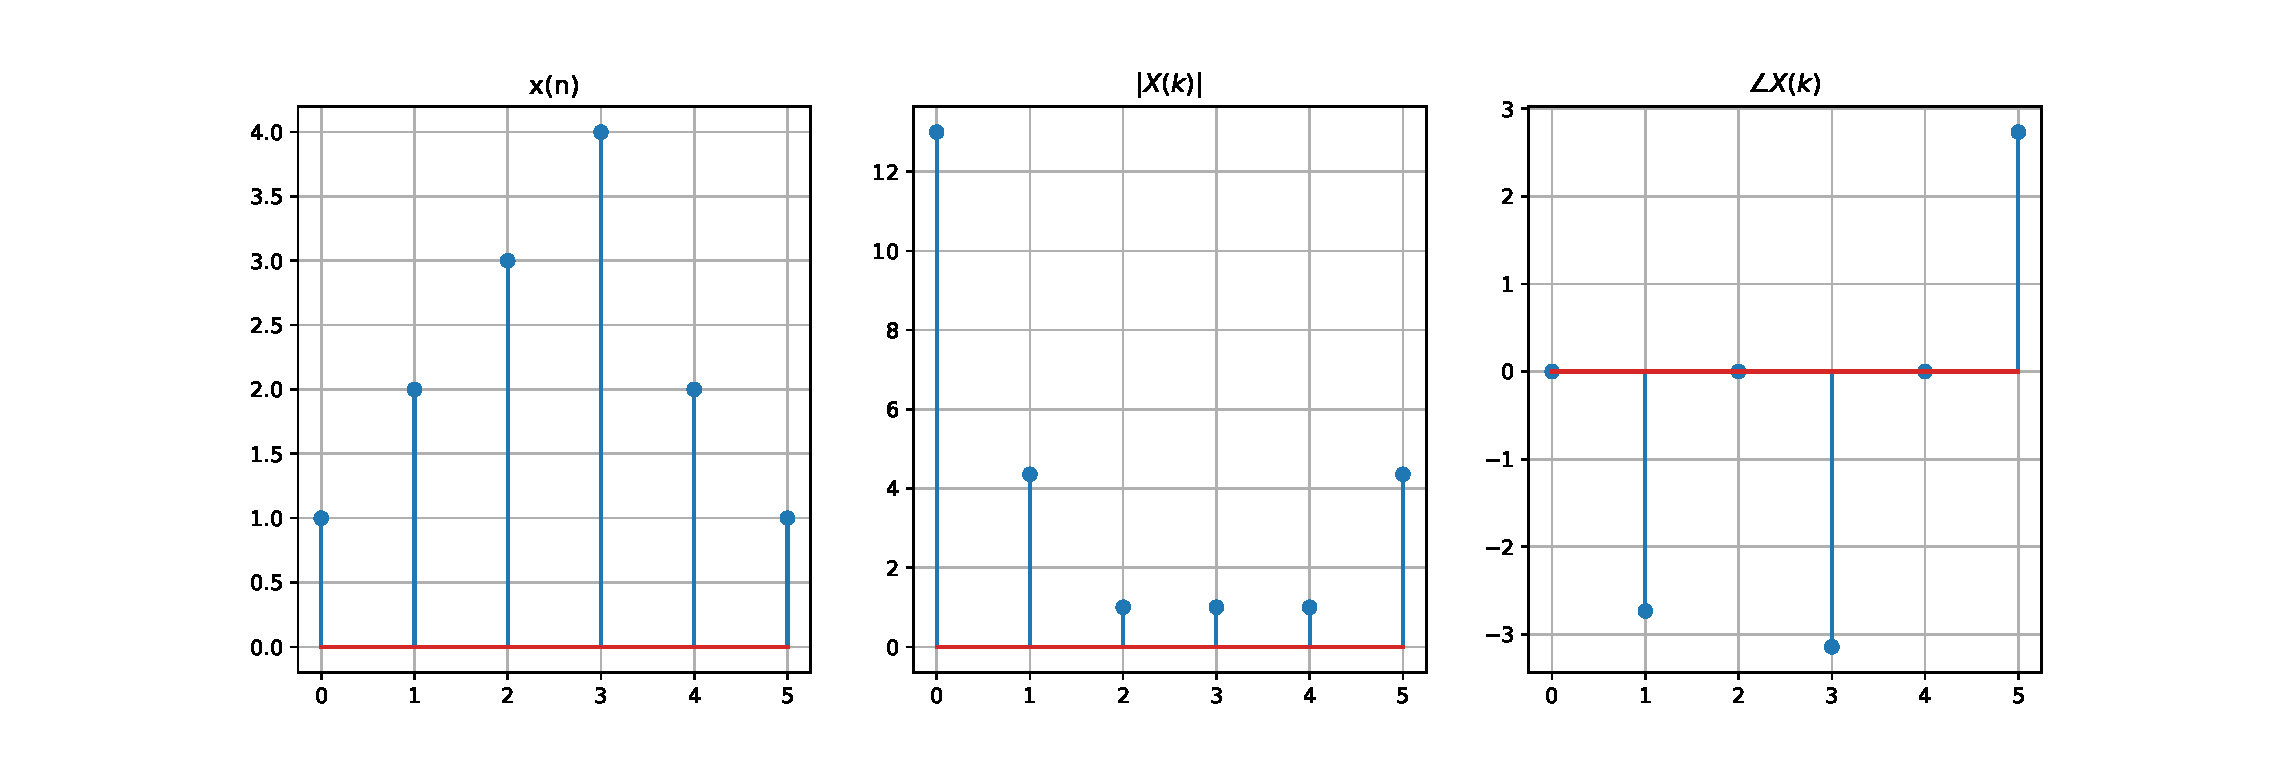
\includegraphics[width=10cm]{./figs/A1_1.eps}
\end{figure}
\begin{figure}[!ht]
	\includegraphics[width=10cm]{./figs/A1_3.eps}
\end{figure}
\begin{figure}[!ht]
	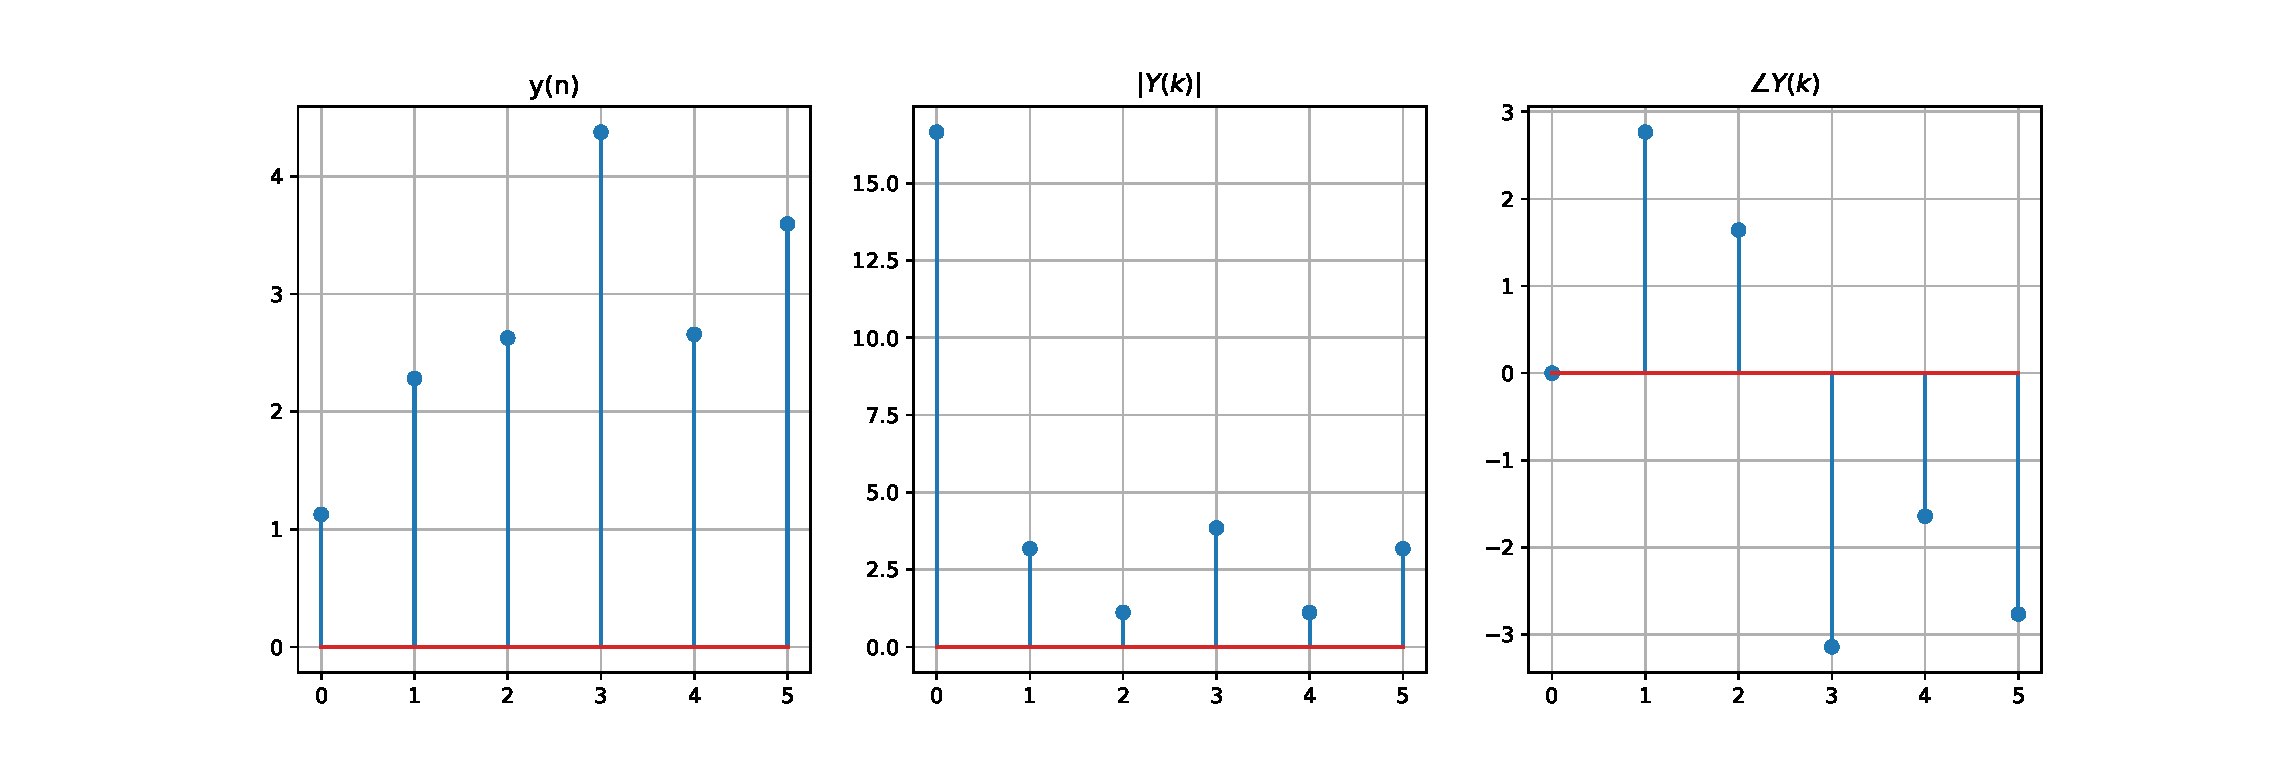
\includegraphics[width=10cm]{./figs/A1_2.eps}
\end{figure}
\item
Benefits of FFT:
\begin{itemize}
    \item The DFT would have $n^2$ operations for the computation, whereas in the modified algorithm (FFT) the number of operations are $2(\frac{n}{2})^2$ since two smaller matrices are combined instead of one large matrix.
    \item Also there is a computational benefit since the matrices are sparse (most elements are zeros or ones). 
    \item If the above is recursively performed, the complexity of the algorithm will be $\frac{n}{2}$logn.
\end{itemize}



\end{enumerate}
\end{document}